\asection{Graph Basics}
\label{Graph Basics}

\setlistdepth{1}


\subsection{Graph Overview}
A Graph in Mathematics and Computer Science is defined as a pair $G = (V, E)$,  where $V$ is the set of vertices and $E$ is the set of edges, formed by pairs of vertices with each other. Figure ~\ref{fig:simplegraph} demonstrates the structural 
attributes of a simple graph.

\begin{figure}[H]
  \begin{center}
      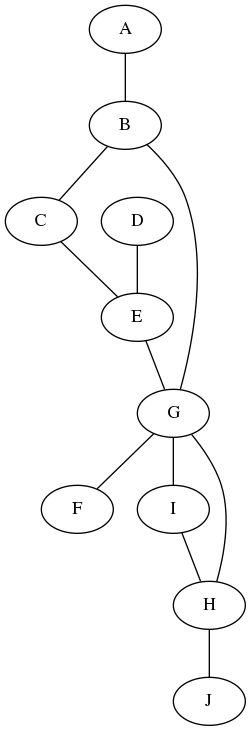
\includegraphics[width=0.2\textwidth]{simplegraph.png}
  \end{center}    
  \caption{Representation of a graph}
  \label{fig:simplegraph}
\end{figure} 
Graphs can either directed or they can undirected. This means that the edges in the graph could have an abscence of direction as in the ~\ref{fig:simplegraph} above, or they could have a direction showing from which
vertice the edge is coming from, and to which vertice the edge is going to. Figure ~\ref{fig:directedgraph} demonstrates a directed graph, commonly known as a digraph. This characteristic is demonstrated by the edge $3$, 
that goes from node $B$ to node $G$, and also by edge 2 that goes from node $B$ to node $C$. 

\begin{figure}[H]
  \begin{center}
      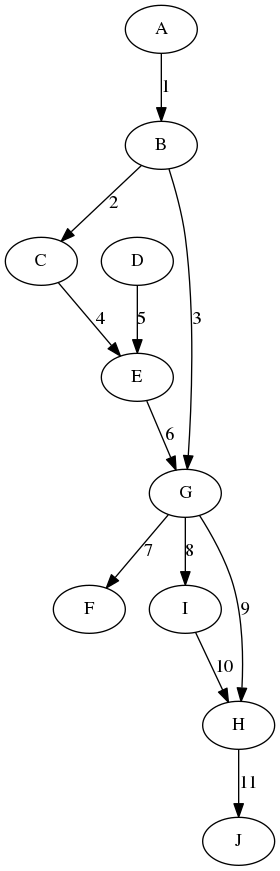
\includegraphics[width=0.2\textwidth]{directedgraph.png}
  \end{center}    
  \caption{Representation of a digraph}
  \label{fig:directedgraph}
\end{figure} 
Note that the undirected graph mentioned above is commonly referred to as a bigraph because the direction
of its edges could be percieved as to going in both direction as it is not specifed.

In this paper, the focus is primarily on directed graphs, and they shall be referred to as digraphs from here onward.


\subsection{Empty graph}
An \textit{Empty graph}, is a graph consisting of \textit{n} vertices and zero edges, where n > 0. An example is demonstrated in the figure \ref{fig:empty_graph}
\begin{figure}[H]
  \begin{center}
      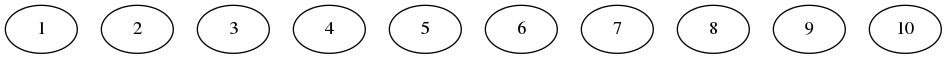
\includegraphics[width=0.65\textwidth]{empty.png}
  \end{center}    
  \caption{Representation of an empty graph with 10 vertices}
  \label{fig:empty_graph}
\end{figure}

In the example above, figure \ref{fig:empty_graph} has 10 vertices but none of the vertices have a relationship with each other thus.

\subsection{Digraph}
A Digraph in mathematics is defined as is a pair of disjoint vertices and edges $(V,E)$, and their repective mappings that comprises of two components, namely the initial vertix and 
terminal vertice of each edge i.e. each edge has a initial vertix: 
  \begin{equation}
    Ei\rightarrow Vi
  \end{equation} 
 and a terminal vertix:

  \begin{equation}
    Vj\rightarrow Ej
  \end{equation} 
   for some vertices $Vi$,$Vj$ in V and edges $Ei$,$Ej$ in E [7] refer to the figure ~\ref{fig:directedgraph}.

\subsection{Graph representation}
Graphs are represented in a variaty of ways, from adjacency lists, incident matrices and adjacency matrices. The algorithms that are studied in this paper make us of adjacency matrices and adjacency list representations of graphs. 

\subsubsection{Adjacency matrices}
An adjacency matrices is a nxn matrix A, with $A(i,j)$ = 1 $iff(i,j) ∈ E$ [9]. This means that wherever there is an edge in the graph, it is denoted by a 1 in the matrix, places in the matrix where there is an absence of an edge, are denoted by 0.\newline\newline
Figure ~\ref{fig:adjacencymatrix} depicts the association between the graph in figure ~\ref{fig:simplegraph} and its adjacency matrix.
\begin{figure}[H]
  \begin{center}
      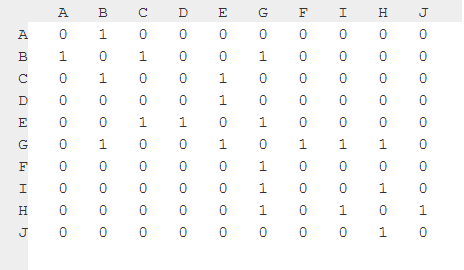
\includegraphics[width=0.65\textwidth]{matrix.png}
  \end{center}    
  \caption{Representation of a graph and its associated adjacency matrix}
  \label{fig:adjacencymatrix}
\end{figure}

\subsubsection{Adjacency list}
An Adjacency list is vertices of a graph, of which each vertice is connected to the list. The vertices in an adjacency list point to their own list of edges that they are connected to(i.e. the list contains the edges that connect them to other vertices). \newpage
Figure ~\ref{fig:adjacencylist} depicts the association between the graph in figure ~\ref{fig:simplegraph} and its adjacency list.
\begin{figure}[H]
  \begin{center}
      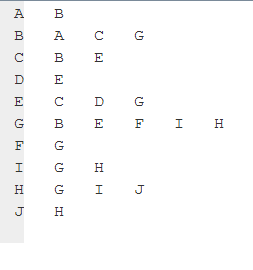
\includegraphics[width=0.4\textwidth]{list.png}
  \end{center}    
  \caption{Representation of a graph and its associated adjacency list}
  \label{fig:adjacencylist}
\end{figure}

\subsubsection{Set of Pairs}
Another representation of graphs is by the use of triplets $(source,destination,lable)$, as depicted in the thesis of Linda Marshall [17] . Each element of the triplet represents a specific attribute of the graph, the first element represent the source vertice, the second represents the destination vertice and the last element represents the corresponding label for the edge.  

\subsection{Supergraphs and subgraphs}
Let $G${\tiny A} be be graph define as follows $G${\tiny A} = ($V${\tiny A},$E${\tiny A}) and let $G${\tiny B} be another graph that is defined as follows $G${\tiny B} = ($V${\tiny B},$E${\tiny B}) where $V${\tiny A},$V${\tiny B} are sets of vertices and $E${\tiny A},$E${\tiny B} are sets of edges.
In graph theory, a graph $G${\tiny A} is said to be a subgraph of graph $G${\tiny B}, and graph $G${\tiny B} is said to be a supergraph of graph $G${\tiny A} if all the vertices and edges that are in graph $G${\tiny A} are also in graph $G${\tiny B}, that is [3]:

\begin{myEnumerate}
  \item $V${\tiny A} $ \subseteq V${\tiny B}, and
  \item Every edge of $G${\tiny A} is also an edge in $G${\tiny B}.
\end{myEnumerate}

In figure  ~\ref{fig:simplegraph}, the graph constructed by vertices $D,E,G,F$ and $I$ is the sub-graph of the entire graph. And thus the graph is a super-graph of the sub-graph constructed by the vertices, namely $D,E,G,F$ and $I$.

\subsection{Graph Isomorphism}
Two graphs are said to be isomorphic if they are syntactically similar to each other $iff$ there is a bijection between their respective nodes which make each edge of $G${\tiny A} correspond to exactly one edge of $G${\tiny B}, and vice versa [12], i.e. the graphs are structurally the same to each other. This property is demonstrated in figures ~\ref{fig:isomorphism}. 
\newpage
The two graphs look very different, but when they are further inspected, it is evident that the two are a representation of the same structural scheme or maybe even the same graph that has been rearranged. \newline\newline Consider the vertice $1$ from the left-most graph, it has three edges going to and from vertices $2,4$ and $5$, and now consider the vertix $a$ from the right-most graph, it also has three vertices going to and from it, namely $g,h$ and $i$. These two vertices have the same structural, but from two different graphs, the same goes for all the other vertices in both graphs .i.e each vertice in the left-most graph can be associtated with one in the right-most graph as we did for vertices $1$ and $a$.

\begin{figure}[!tbp]
  \begin{subfigure}[b]{0.2\textwidth}
    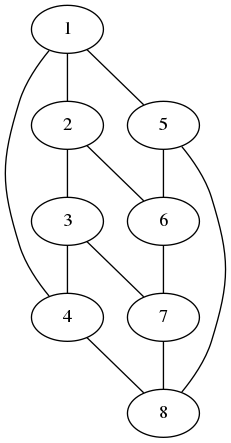
\includegraphics[width=\textwidth]{isomorphismleft}
    \caption{Isomorphic graph on the left}
    \label{fig:isomorphism}
  \end{subfigure}
  \hfill
  \begin{subfigure}[b]{0.4\textwidth}
    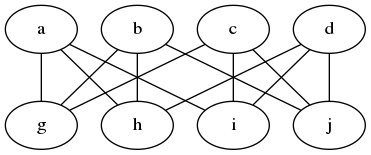
\includegraphics[width=\textwidth]{isomorphismright}
    \caption{Isomorphic graph on the right}
    \label{fig:isomorphism}
  \end{subfigure}
  \caption{A demostration of two isomorphic graphs}
\end{figure}

\newpage